\subsection{Variables and possible positions}
\label{subsec:poss_poses}
Now is a good time to discuss then how to represent a path through an energy landscape as a factor graph, and how to define those potential functions to give a higher probability to good paths.
It makes sense for the variable nodes to represent the points along the path, and then for the possible values they can take to represent the positions they can be in the space.
Continuous MRFs do exist but they are not well suited to this problem, hence we also need to pick for each variable (variable node) a finite number of discrete positions it can take.

There are plausibly many possible ways of doing this, the approach that we use seems a reasonable way to create a set of points in a manner that can scale to arbitrary $D$ dimensions.
You need to define a set of points that most paths would travel through between the two minima.
The algorithm as currently implemented creates a hypersphere of points around the midpoint between the two minima, with the sphere's diameter being slightly wider than the gap between the two points.
In order to do this it creates a hypercube grid of points wider than the sphere will be, with $S$ points along each edge.
Increasing $S$ will create a more detailed path, but it will also increase complexity, especially in high dimensions where the number of points being considered will be approximately $S^D$.

The points are also rotated so that the points can be split into slices orthogonal to the vector that connects the two minima.
This is achieved by creating the hypercube in a non-standard basis where the first basis vector is in the direction of the minima line, and then transforming it back into the standard basis.
You can see the exact implementation in the code, but the results are displayed in Figure~\ref{fig:points_samp} for $D=2$ and $D=3$.

\begin{figure}[h]
\centering
\begin{subfigure}{.5\textwidth}
  \centering
  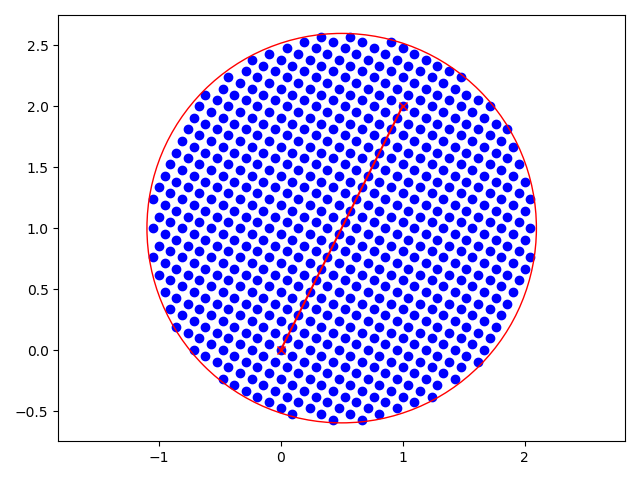
\includegraphics[width=\linewidth]{Circle Sampling.png}
  \caption{Sampling in 2D}
  \label{fig:circ_samp}
\end{subfigure}%
\begin{subfigure}{.5\textwidth}
  \centering
  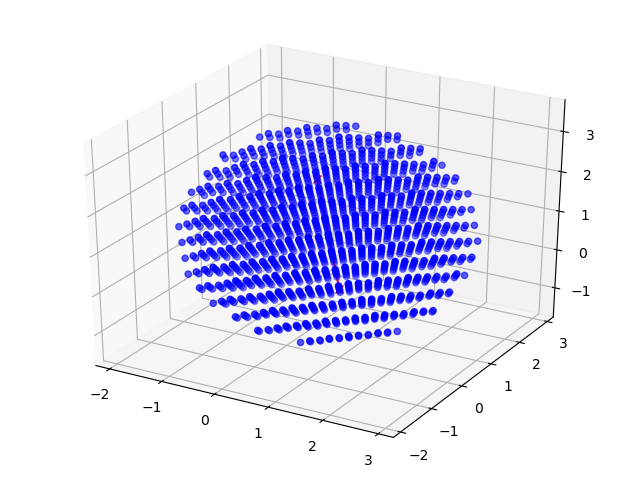
\includegraphics[width=\linewidth]{Sphere Sampling.png}
  \caption{Sampling in 3D}
  \label{fig:sphere_samp}
\end{subfigure}
\caption{How the sampling algorithm performs in 2D and 3D. Red crosses connected by a red line denote the two minima that the path will connect, but it is quite difficult to spot in the sphere!}
\label{fig:points_samp}
\end{figure}

We should not, however, let every variable along the path take every position in the sphere.
It would be ridiculous for the path to jump to one end of the sphere and then jump back, and furthermore allowing each variable more possible values increases computational complexity.
Therefore we restrict the variables to only take values in a slice of the sphere, with one slice for each variable representing one section of the path, as in Figure~\ref{fig:slice_samp}.

\begin{figure}[h]
    \centering
    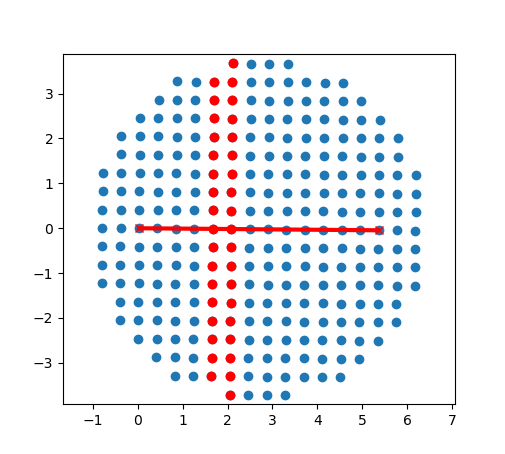
\includegraphics[width=.5\linewidth]{slicing.png}
    \caption{The points generated for a sphere (blue) with the points that are in one variable's slice highlighted in red. In addition the two minima are marked with a red x and connected by a red line. As you can see the slice is perpendicular to the minima direction.}
    \label{fig:slice_samp}
\end{figure}

Already at this point the algorithm has a lot of customisable parameters.
You can decide how wide you want your slices to be, how many variables you want spanning the gap between the two minima, how many point positions you want spanning the gap between the two minima, how much the slices overlap with each other (slices can overlap but it will increase computational complexity a little bit), how much wider to make the sphere of points than the gap between the two minima.
The code can even make the sphere a sphereoid, stretched in certain directions so that you can explore more of the energy landscape.
There is no easy way to evaluate how much effect changing these parameters has on path quality, although the effect on time complexity is more obvious.

In general, for the code we use later, the number of variables was 5, the number of positions spanning the gap between the two minima was 5 and the width of a layer was 1, no overlap, spherical shape.
This level of parameters produced decent parameters and ran quickly enough to allow a lot of samples of even higher dimensional problems.
In addition it produced acceptable results when checked manually in lower dimensions (the same was not true of reducing the number of variables or points spanning the gap to 4, which seems to be too coarse).

We also add a variable at the start and end of the paths to represent the start and end positions, however we only allow these nodes to be at one position, the start and end position respectively. 
This tethers our paths at the ends.

\FloatBarrier
\subsection{Factors and quality functions}
\label{subsec:fac_qual}
Next we need to choose how we arrange our factors and with it how we choose our potential functions to give the highest weight to good paths.
For the factor arrangement it may seem optimal to just connect a factor to every single variable, and from there define a clever function that gives high scores to very good paths by considering the whole path.
However we will see later that the MPMP algorithm requires that we reduce as far as possible how many variables each factor node is connected to.
It also requires that our factor graph doesn't have any cycles in it, making it a factor tree.
Therefore we connect each variable node to its neighbor, creating a chain from the start of the path to the end, with no other connections.
You can see an example of a path factor tree generated by the MPMP algorithm in Figure~\ref{fig:path_ftree}.

\begin{figure}[h]
    \centering
    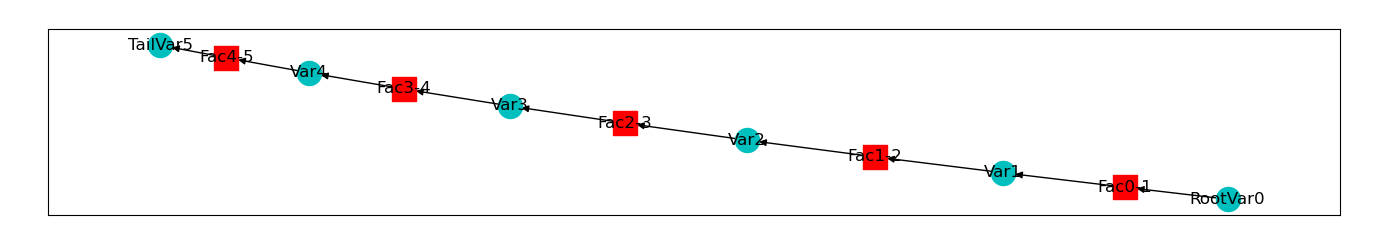
\includegraphics[width=\linewidth]{Short ftree structure.png}
    \caption{A computer visualisation of the factor tree generated for the MPMP algorithm, with variables as circles and factors as squares.}
    \label{fig:path_ftree}
\end{figure}

That then leaves the question of how to define the factor potentials or qualities.
The primary aim of the path is to reduce the maximum energy level it goes through, however the path must also go through the minimum possible energy path to get to that max energy point.
Furthermore the path must not be excessively long.

As you will recall, the quality of the overall path is the product of the quality of each factor, and each factor can only take into account the nodes it is connected to.
We use a linear combination of different features to create a score for the transition.
Features measure one aspect of the quality of the transition, for example there is one feature that penalises jumps that are longer so that paths are reluctant to take large jumps.
Qualities must be at least zero however, so to allow score to be any value, we take the exponent of the score.

Let the start point of a feature be $\mathbf{x}_0$ and the end point $\mathbf{x}_1$, with start meaning the point in the path is closer to the beginning of the path, and moving on to the end point which is further down.
Let $a_0, a_1, \mathellipsis, a_{n_f} \in \mathbb{R}$ be the coefficients for the features $f_0, f_1, \mathellipsis, f_{n_f} \in \mathbb{R}^D \times \mathbb{R}^D \mapsto \mathbb{R}$.
In equation form the potential for factor F is
\begin{equation}
    \label{eq:factor_qual}
    \phi_F(\mathbf{x}_0, \mathbf{x}_1) = \exp(a_0 f_0(\mathbf{x}_0, \mathbf{x}_1) + a_1 f_1(\mathbf{x}_0, \mathbf{x}_1) + \mathellipsis + a_{n_f} f_{n_f} (\mathbf{x}_0, \mathbf{x}_1)).
\end{equation}

Let $E(\mathbf{x})$ be the energy strength at point $\mathbf{x}$.
Let $\mathbf{x}_{0.5} = (\mathbf{x}_0 + \mathbf{x}_1) / 2$ be the midpoint of the two points.
The features we tested for the score were (with their names in (brackets))
\begin{itemize}
    \item (Length) minus the length of the transition
    \begin{itemize}
        \item $-|\mathbf{x}_0 - \mathbf{x}_1|$
        \item This means that longer jumps are given lower scores.
        \item In general the length is scaled by how far apart the points in the grid are so that the algorithm works well in different situations and settings.
        \item Turned up to high this would make the algorithm "cut corners", and go in as straight a line as possible between the minima, so we tended to keep this feature near zero anyway.
    \end{itemize}
    \item (Length Cutoff) a score of $-\infty$ if the path's length is over a chosen cutoff
    \begin{itemize}
        \item This prevents truly crazy jumps, as that jump will have quality zero.
        \item In addition, you can code it so it reduces the number of calculations the algorithm has to do.
        By eliminating far away points the algorithm has fewer combinations of points to consider, saving time.
    \end{itemize}
    \item (Strength) minus the average energy of the midpoint and endpoint
    \begin{itemize}
        \item $-(E(\mathbf{x}_{0.5})+E(\mathbf{x}_1))$
        \item This makes the path favor going through lower energies.
        \item It has the negative side effect of making the path stay in areas of low energy even if it then forces them to go through a relatively high energy maximum path energy later.
        \item The midpoint energy is calculated so that if the MPMP algorithm is run with coarse settings (not many points) it can't "jump" over a high energy area without paying a cost.
        \item The start point is not used because then the end points of the path would be double counted in different factors.
    \end{itemize}
    \item (Strength Diff) minus the energy increase from the start point to the highest of the midpoint or the endpoint, 0 if the energy is decreasing from the start point.
    \begin{itemize}
        \item $-(\max(E(\mathbf{x}_1), E(\mathbf{x}_{0.5})) - E(\mathbf{x}_0))$ if the energy is increasing from $\mathbf{x}_0$ else 0, aka this feature is at most 0.
        \item Gives a negative score to a big energy increase from the start node, so tries to reduce the maximum energy that the path goes through.
        \item When you take the product of all the factor qualities it will be the exponent of the sum of all the factor scores.
        If the path goes uniformly up and then uniformly down, then the sum of the strength diff scores will be the maximum point the path goes through, minus the initial starting energy.
        \item Hence, this feature minimises the maximum strength the path goes through.
        \item This feature only takes into account the highest point the path goes through, therefore relying on this feature alone can lead to paths that do have a low maximum, but take a terrible path to get there.
        \item In addition, this feature might favor skirting along the mountainside of a valley when it should be falling down into the centre of the valley, if it prevents the path from dipping down and going back up again.
        This is because the "going back up again" part will be penalised by this feature.
    \end{itemize}
    \item (Gradient) the length of the grad vector at the midpoint, after making the gradient vector orthogonal to the direction of the path.
    \begin{itemize}
        % cite a way of getting the gradient
        \item This feature was borrowed from the Nudged Elastic Band method.
        In Nudged Elastic Band they make the path fall down the slope into the valleys by pushing the points of the path down the gradient of the Energy scalar field.
        However, they only let the points be pushed in the direction orthogonal to the path, so that the points could stay equidistant to each other.
        When you're in a valley moving between the minima on the minimum energy pathway your path will have gradient zero in every direction, because otherwise you would be able to move to get a lower path.
        Every direction that is, except the direction of the path, because it may need to be moving up a gradient to be getting to a goal in the direction of the path.
        \item This feature is meant to incentivise a small orthogonal gradient, meant to favor paths at the bottom of the valley.
        \item This feature did not work well, because in addition to favoring the bottom of the valley the feature also favors the ridge of a hill, since using the first derivative alone cannot distinguish between a minima and a maxima.
        See Figure~\ref{fig:grad_incorrect} for an example.
    \end{itemize}
    \begin{figure}[h]
        \centering
        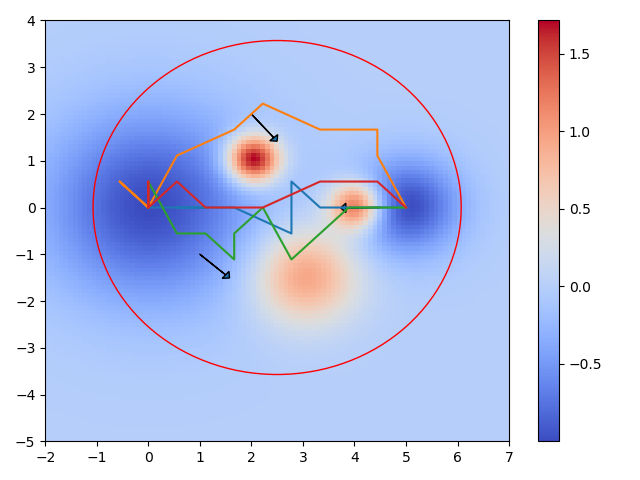
\includegraphics[width=.7\linewidth]{incorrect paths.png}
        \caption{A selection of MPMP generated paths with the gradient feature on (no second order). You can see that the green and blue paths head directly for the maxima.}
        \label{fig:grad_incorrect}
    \end{figure}
    \item (Second Order) the second order derivative in the direction of the orthogonal component of the gradient.
    \begin{itemize}
        \item This feature was added to stop the issue of the first order derivative favoring maxima, by favoring a second order derivative that was high (a minima).
        \item It turned out to be a non-ideal feature because it would draw the path to strange areas of the energy landscape that happened to have high second derivatives.
        \item It also required a lot of extra computation, which made the algorithm a lot slower.
    \end{itemize}
\end{itemize}

Overall, out of these features, we only used Length Cutoff, Strength and Strength Diff.
For the reasons mentioned above, the gradient based and length features were ineffective.
We discovered the strength and strength diff feature needed to be scaled so that in environments with dramatically different energy levels they would perform similarly.
We would take a scan of the energy along the straight line between the two minima and rescale all the energies such that the max seen on that line was an energy of 1 and the minimum was 0 $E_{\text{rescaled}} = (E - E_{\min})/(E_{\max}-E_{\min})$.

We are not yet done with deciding quality features, as we need to decide the relative weights of the features in the linear combination that makes up the score (the $a_0, a_1, \mathellipsis$ from~\eqref{eq:factor_qual}).
We tried out the algorithm on 2D and 3D environments where the best paths were obvious, and deduced good settings from this experimentation.
The length feature should be near zero, but keep the length cutoff on.
Strength should have tuning coefficient 1 and Strength Diff tuning coefficient 1.5.

The best method of evaluating the paths was to create a function that would take in the paths produced by the algorithm and print the factor by factor and overall scores for each feature.
This made it very obvious which features were most influencing the path.
It was ideal to have the Strength Diff feature about 25\% larger than the Strength feature.
This meant the algorithm would first prioritize reducing the path's maximum point, but could also secondarily focus on reducing the path's energy in how it got to that minimised max (minimax) point.

Now we have a way to define paths as an MRF and evaluate a path's quality, we can now look at the algorithm to maximise the quality.

\FloatBarrier